\section{Реализация моделей}
	В данном разделе приводится краткое описание программной реализации
	моделей, примеры результатов идентификации частотных сканов, рассматриваются 
	некоторые методические вопросы.


	\subsection{Интерфейс и функционал}
	Модели оформлены в виде пакета модулей на языке программирования Python~3.
	Интерфейс моделей совместим с одной из самых популярных библиотек для 
	машинного обучения scikit-learn \cite{sklearn_website}. Такое техническое
	решение позволяет использовать имеющиеся в библиотеке инструменты 
	предобработки данных, оценки качества и оптимизации параметров 
	моделей, а также интегрировать модели в друге программное обеспечение.

	Разработанные модели (выражения	\ref{eq:dls82e_model_S_short}, 
	\ref{eq:dls82e_model_S_p}, \ref{eq:multiexp_frequncy_scan}), выполняют две 
	функции:
	\begin{enumerate}
		\item Вычисление частотного скана с заданными параметрами.
		\item Идентификация параметров модели частотного скана по 
		экспериментальным данным.
	\end{enumerate}
	Идентификация параметров моделей реализована методом градиентного спуска.
	Имеется возможность вывода значений параметров модели на каждой итерации.
	Реализована автоматическая остановка идентификации при достижении заданного
	модуля разности между значениями функции потерь на текущей и предыдущей 
	итерации.

	Модели реализуют единообразный интерфейс. При инициализации каждая модель 
	получает длительность импульса заполнения (параметр filling\_pulse),
	которая считается неизменной при измерениях) и параметры алгоритма 
	идентификации. Параметры алгоритма идентификации варьируются:
	\begin{itemize}
		\item модель идеального частотного скана и модель частотного скана с 
		показателем нелинейности-неэкспоненциальности (выражения 
		\ref{eq:dls82e_model_S_short}, \ref{eq:dls82e_model_S_p}): 
			\begin{description}
				\item[fit\_p\_coef] -- если параметр принимает значение True 
				(логическую единицу), тогда при идентификации параметров модели
				определяется показатель нелинейности-неэкспоненциальности $p$,
				иначе (False -- логический ноль) $p$ считается равным 1 и не 
				изменяется при идентификации параметров модели;
				\item[learning\_rate] -- скорость градиентного спуска;
				\item[n\_iters] -- максимальное количесво итераций при 
				идентификации;
				\item[stop\_val] -- модуль разницы между значениями функции 
				потерь на текущей и предыдущей итерации, при достижении которого
				происходит остановка идентификации;
				\item[verbose] -- если параметр принимает значение True, то в 
				стандартный поток вывода печатаются значения параметров модели
				на каждой итерации.
			\end{description}

		\item модель многоэкспоненциального частотного скана (выражение 
		\ref{eq:multiexp_frequncy_scan}):
			\begin{description}
				\item[n\_exps] -- количество экспоненециальных составляющих в 
				сигнале релаксации (значение $n$ в выражении 
				\ref{eq:multiexp_frequncy_scan});
				\item[learning\_rate] -- скорость градиентного спуска;
				\item[n\_iters] -- максимальное количесво итераций при 
				идентификации;
				\item[stop\_val] -- модуль разницы между значениями функции 
				потерь на текущей и предыдущей итерации, при достижении которого
				происходит остановка идентификации;
				\item[verbose] -- если параметр принимает значение True, то в 
				стандартный поток вывода печатаются значения параметров модели
				на каждой итерации.
			\end{description}
	\end{itemize}

	При идентификации параметров модели идеального частотного скана 
	определяется амплитуда и десятичный логарифм постоянной времени 
	($\log_{10}(\tau)$) сигнала релаксации. Причины замены постоянной времени
	её десятичном логарифмом объясняются в следующем разделе.

	При идентификации модели с показателем нелинейности"=неэкспоненциальности
	к амплитуде и десятичному логарифму постоянной времени сигнала релаксации
	добавляется значение показателя нелинейности"=неэкспоненциальности $p$.

	При идентификации многоэкспоненциальной модели определяется $n$ пар 
	амплитуда --- десятичный логарифм постоянной времени сигнала релаксации. 
	По паре для каждой из $n$ экспоненциальных составляющих.

	Параметры модели частотного скана могут быть не только идентифицированны,
	но и заданы пользователем.

	Чтобы выполнить идентификацию параметров модели, нужно передать ей 
	набор экспериментальных (тренировачных) данных, состоящих из вектора 
	значений десятичных логарифимов частоты опорной функции ($\log_{10}(F_0)$)
	и соответствующего вектора значений сигнала DLTS -- сигнала на выходе 
	аппаратного тракта спектрометра DLS-82E. При идентификации параметров модели
	по умолчанию их начальные параметры выбираются случайным образом, однако
	могут быть и определены пользователем.

	При идентификации модели значения её параметров на каждой итерации 
	сохраняются в атрибуте fit\_results\_, что позволяет пользователю
	получить и проанализировать данные о работе алгоритма идентификации.

	При вычислении частотного скана с заданными параметрами модели передаётся
	вектор значений десятичных логарифимов частоты опорной функции, для каждого 
	из которых модель вычислит значение сигнала	DLTS.


	\subsection{Алгоритм идентификации параметров моделей}
	Идентификация параметров модели производится методом градиетного 
	спуска, при этом минимизируется среднеквадратическая ошибка между 
	значениями, полученными в результате измерений, и результатами 
	моделирования (выражение \ref{eq:mse}).
	\begin{equation}
		\label{eq:mse}
		E = \frac{1}{m}\sum_{i=1}^{m}\left(y_i - y_i^*\right)^2,
	\end{equation}
	где
	\begin{description}
		\item[$y_i$] -- значения, полученные в результате измерений,
		\item[$y_i^*$] -- значения, полученные в результате моделирования,
		\item[$m$] -- количество измерений.
	\end{description}
	При каждом обновлении постоянной времени сигнала релаксации (как при 
	идентификации модели, на каждой итерации, так и при обновлении постоянной 
	времени пользователем) вычисляется масштабный множитель $M(\tau, F_0, t_1)$, 
	определяемый выражением \ref{eq:dls82e_model_M}. Таким образом модель 
	всякий раз вычисляет значение 	
	\(
		\max{\left[
	    \tau F_0 e^{-\frac{0.05}{\tau F_0}}
	    \left(1-e^{\frac{t_1 F_0-0.45}{\tau F_0}}
	    -e^{-\frac{0.5}{\tau F_0}}+
	    e^{\frac{t_1 F_0-0.95}{\tau F_0}}\right)
	    \right]}
    \).
    В текущей реализации моделей данный максимум вычисляется приблизительно
    с помощью градиентного спуска. Не смотря на то, что применяемый итеративный
    алгоритм находит максимум очень быстро, эти вычисления занимают довольно 
    много веремени при идентификации моделей, потому что выполняются на 
    каждой итерации (при каждом обновлений постоянной времени $\tau$). В случае 
    многоэкспоненциальной модели данный процесс повторяется еще и для каждой 
    экспоненциальной составляющей, что заметно снижает скорость идентификации 
    модели при значениях параметра n\_exps больше 10. Таким образом в будущем 
    вычисления можно будет оптимизировать за счёт одного из следющих решений:
    \begin{enumerate}
    	\item найти точное аналитическое выражение для расчёта 
    	$M(\tau, F_0, t_1)$,
    	\item найти для $M(\tau, F_0, t_1)$ аппроксимирующую функцию, 
    	позволяющую вычислять мастабный множитель с приемлимой точностью.
    \end{enumerate}

	В моделях градиентный спуск реализован при помощи библиотеки TensorFlow
	\cite{tf_website}, главное преимущество которой в том, что она реализует
	алгоритм автоматического дифференцирования на графе вычислений. Таким 
	образом, при расчёте градиентов сначала производные берутся символьно 
	(точно), а затем вычисляются их значения, поэтому точность вычисления 
	градиента ограничена только разрядностью чисел \cite{hands_on_ml},
	\cite{nikolenko_deep_learning}, \cite{tf_website}.

	Во всех моделях используется алгоритм идентификации с постоянной и одинаковой
	для всех параметров скроростью градиентного спуска, поэтому для ускорения 
	идентификации параметров моделей и улучшения сходимости алгоритма необходима 
	нормализация (прведение к единому масштабу) тренировочных данных.
	
	\begin{figure}[!htp]
		\centering
		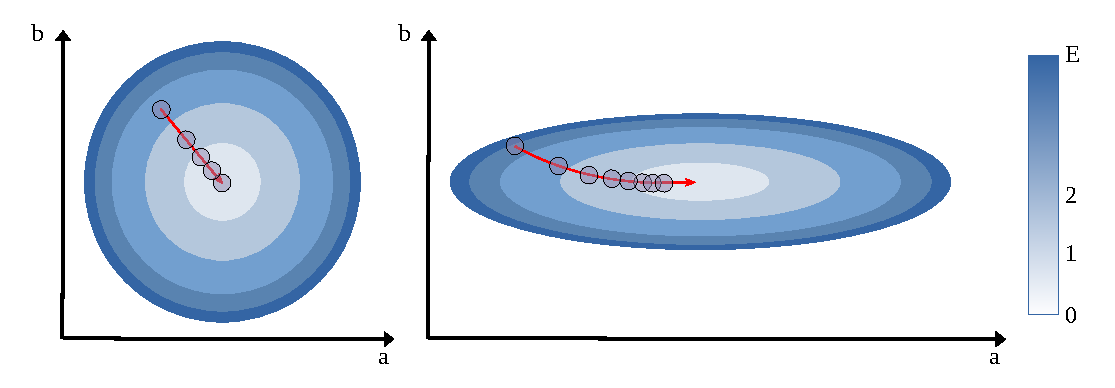
\includegraphics[width=\textwidth]{path_example}
		\caption{Градиентный спуск с нормализацией тренировачных данных (график
		слева) и без неё (график справа) для модели с двумя параметрами. $a$ и 
		$b$ -- параметры модели, $E$ -- функция потерь.}
		\label{pic:path_example}
	\end{figure}

	Рассмотрим примеры на рисунке \ref{pic:path_example}. В идеальном случае 
	функция потерь (среднеквадратическая ошика -- выражение \ref{eq:mse}) должна
	иметь форму <<симметричной чаши>>, а изменение обоих параметров должно вносить 
	одинаковый вклад в значение градиента. В таком случае алгоритм градиентного 
	спуска достигнет минимума функции потерь кратчайшим путём, как на левом 
	графике рисунка \ref{pic:path_example}. Если же тренировочные данные имеют
	очень разные масштабы, функция потерь (гафик справа на рисунке 
	\ref{pic:path_example}) будет иметь форму <<вытянутой чаши>>, а алгоритм 
	идентификации будет долго подстраивать одни из параметров без существенного
	изменения функции потерь \cite{hands_on_ml}. Чтобы минимизировать этот 
	эффект,	тренировочные данные нормализуют перед идентификацей параметров 
	модели. После идентификации параметры модели и тренировочные данные можно
	вернуть в исходный масштаб.

	Для разрабатанных моделей тренировочные данные данные имеют существенно
	отличающиеся масштабы: значение сигнала DLTS находятся в диапазоне долей
	пикофарад, а диапазон изменения частоты опорной функции спектрометра
	покрывает три декады (от 1 Гц до 2500 кГц). Таким образом, желательно 
	выполнять нормализацию исходных данных перед идентификацией параметров
	модели. Кроме этого, изменение параметров модели (постоянной времени и 
	амплитуды) вносят существенно различающийся вклад в градиент функции потерь.
	Если снова обратиться к выражениям \ref{eq:dls82e_model_phi} и 
	\ref{eq:dls82e_model_S_short}, можно заметить, что значение функции потерь
	пропорционально первой степени амплитуды $A$ сигнала релаксации и экспоненте,
	возведенной в степень скорости экспоненциального спада, то есть
	$e^\frac{1}{\tau}$. Поэтому на вход моделей при идентификации подаётся 
	десятичный логарифм частоты опорной функции ($\log_{10}(F_0)$), а 
	идентификация производится не по постоянной времени $\tau$, а по десятичному
	логарифму постоянной времени $\log_{10}(\tau)$. На рисунке \ref{pic:path}
	показан приемер идентификации идельного частотного скана. <<Путь>> 
	параметров модели в процессе идентификации показывает красная линия с 
	маркерами, а изолинии и градиент -- значения функции потерь.

    \begin{figure}[!htp]
        \centering
        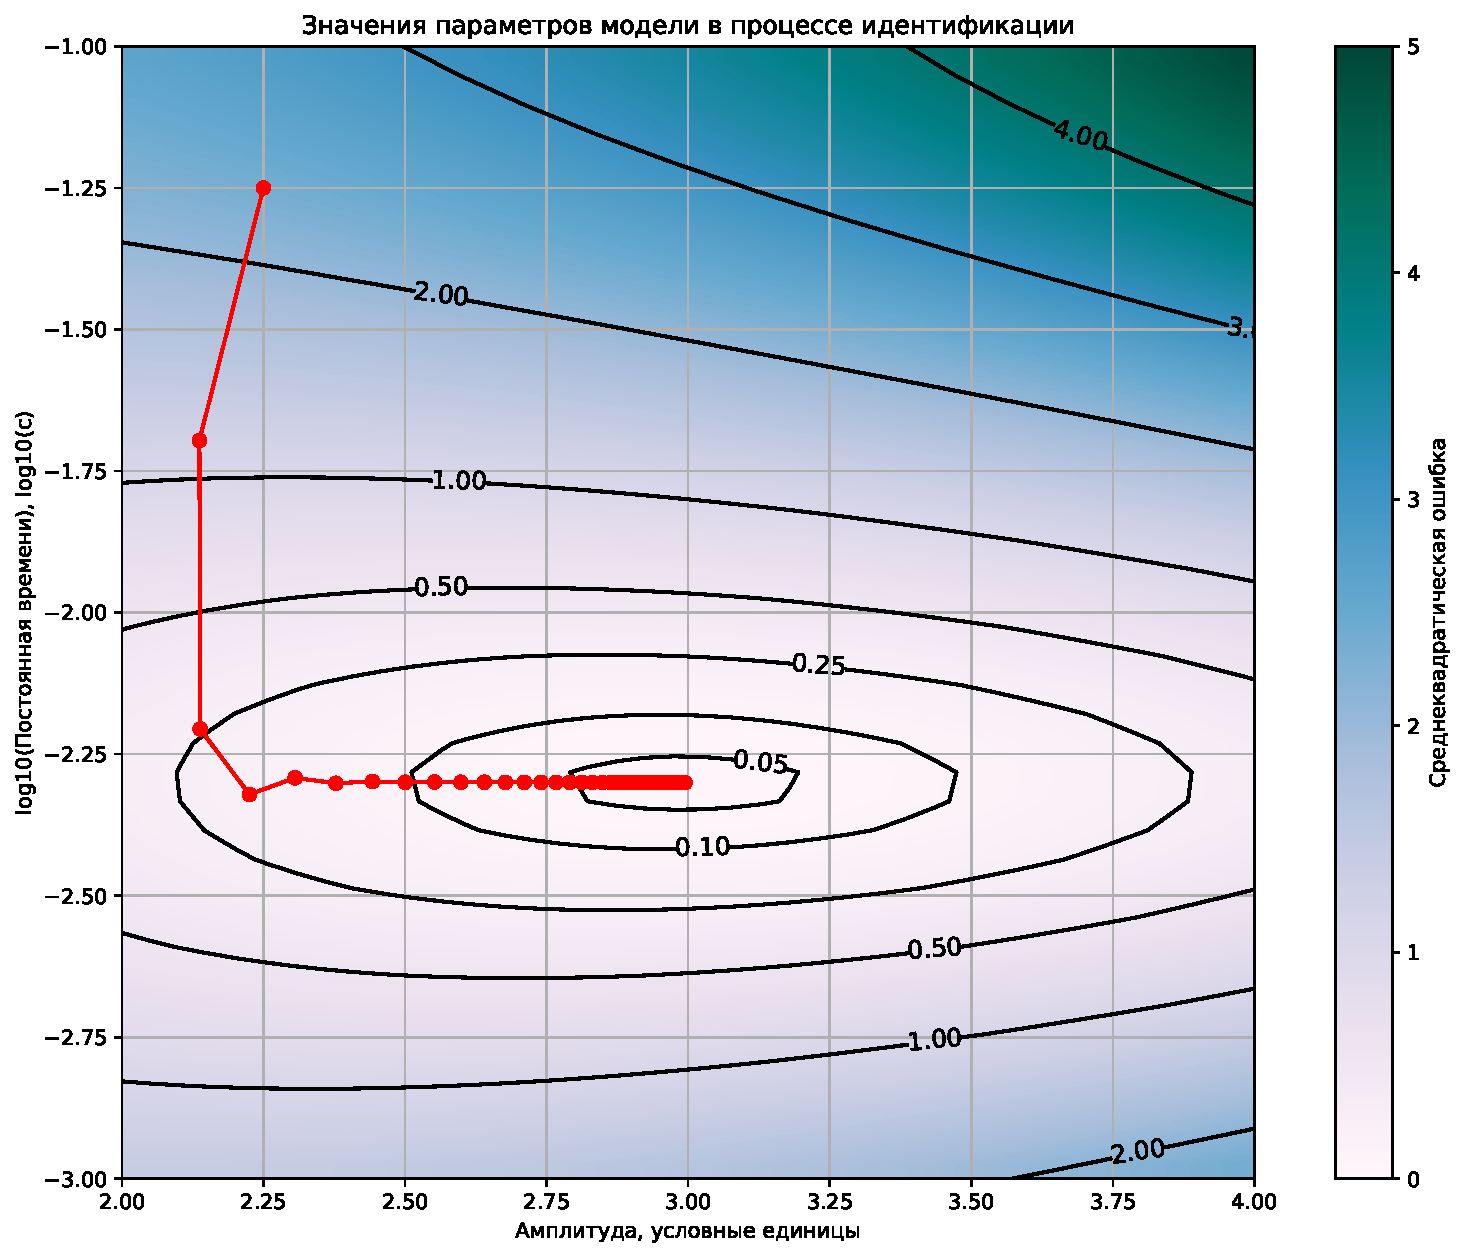
\includegraphics[width=0.75\textwidth]{path}
        \caption{<<Путь>> значений параметров при идентификации.}
        \label{pic:path}
    \end{figure}

    На рисунке \ref{pic:path} форма изолиний отличается от концентрических 
    окружностей, а <<путь>> параметров не похож на прямую линию, что говорит
    о том, что возможна дальнейшая оптимизация алгоритма идентификации, однако,
    названные выше меры позволили значительно смягчить эффект от различных 
    масштабов в экспериментальных данных и в параметрах модели. Также возможно
    использование одного из алгоритмов адаптивного градиентного спуска, то есть
    алгоритмов изменяющих скорость по мере приближения к оптимальным значениям
    параметров. Такое решение не изменит форму функции потерь, но оптимизирует
    <<путь>> и количество итераций.

    Рисунки \ref{pic:identification_test} и \ref{pic:multiexp_test} показывают
    примеры результатов идентификации модели идеального частотного скана и 
    модели многоэкспоненциального частотного скана соответственно на 
    расчитанных тренировочных данных.

    \begin{figure}[!htp]
        \centering
        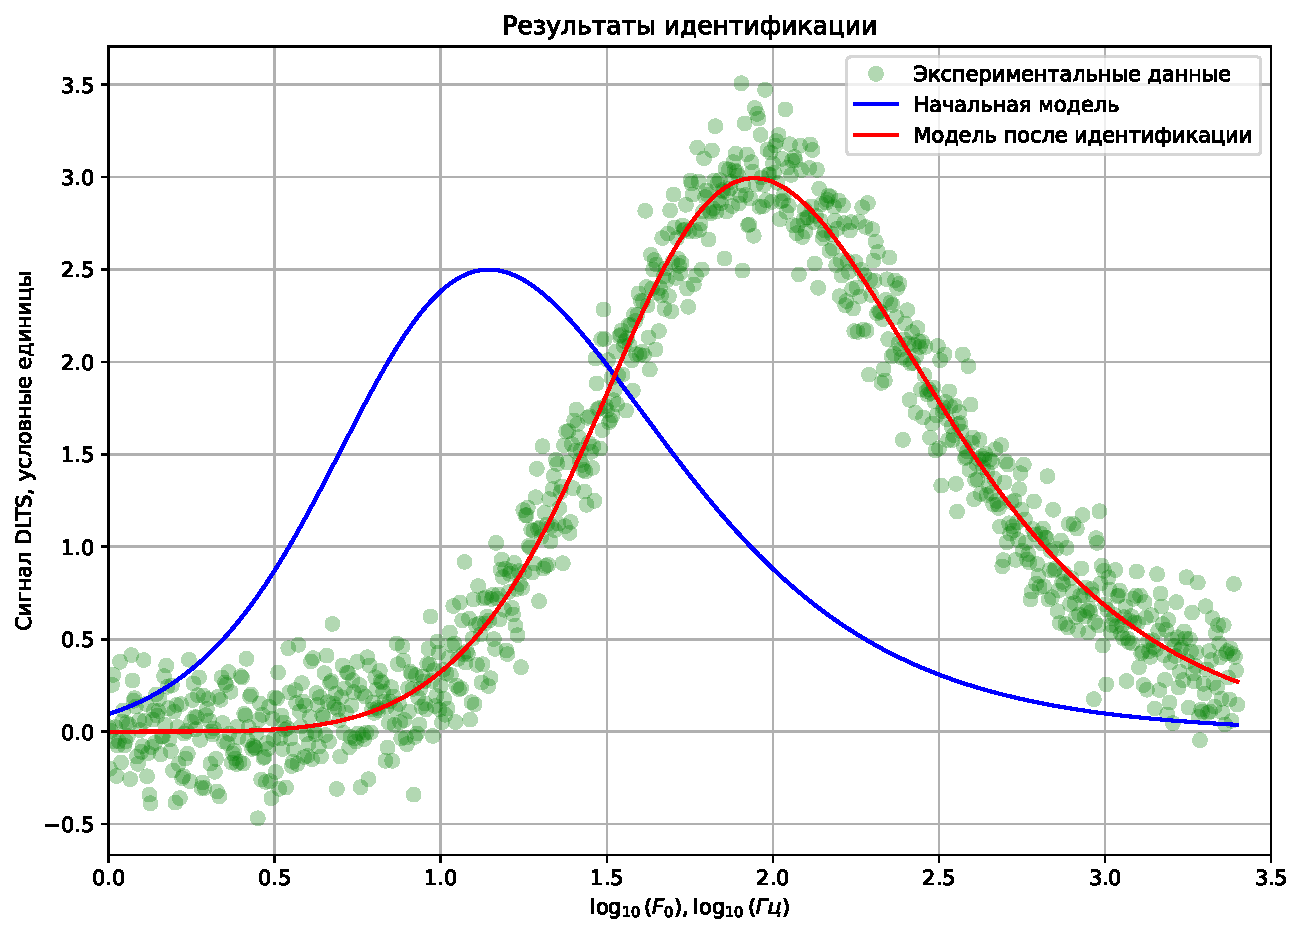
\includegraphics[width=0.75\textwidth]{identification_test}
        \caption{Пример результата идентификации модели идеального частотного 
        скана.}
        \label{pic:identification_test}
    \end{figure}


    \begin{figure}[!htp]
        \centering
        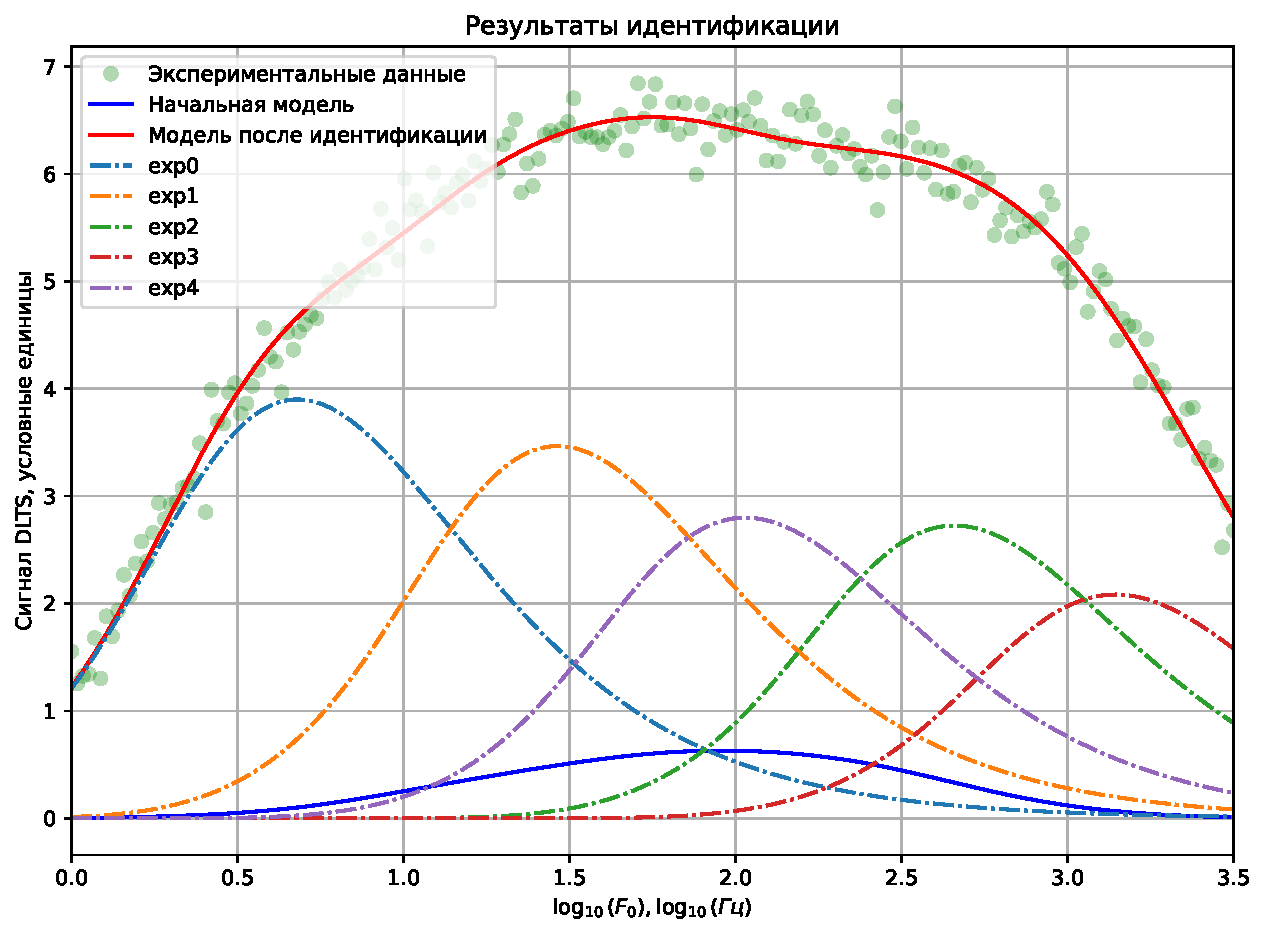
\includegraphics[width=0.75\textwidth]{multiexp_test}
        \caption{Пример результата идентификации модели многоэкспоненциального
        частотного скана. Штрихпунктирными линиями показаны частотные сканы для
        отдельных экспоненциальных составляющих сигнала релаксации.}
        \label{pic:multiexp_test}
    \end{figure}


    \subsection{Оценка качества модели}
    Вычисление корня из среднеквадратической ошибки (англ. root-mean-square 
    error -- RMSE) между экспериментальными данными и данными, полученными с 
    помощью моделирвоания, -- один из самых известных и распространенных 
    способов оценки качества регрессии данных разработанной моделью. Однако, 
    одного этого показателя часто бывает недостаточно, более того, 
    \textbf{оценка этого показателя только на тренировочных данных} при 
    разработке модели (\textbf{особенно эмпирической модели}) -- методическая 
    ошибка \cite{hands_on_ml}, \cite{sklearn_cross_validation}. Данные 
    утверждения обусловлены следующим:
    \begin{itemize}
    	\item сам по себе корень из среднеквадратической ошибки не отвечает на 
    	вопрос о <<фундаментальном>> соответствии данных модели, а также не 
    	показывает какова вероятность того, что полученное значение -- результат 
    	случайного совпадения;
    	\item оценивая данную метрику только на тренировочных данных, есть риск
    	получить слишком оптимистическую оценку и столкнуться с проблемой, 
    	называемой <<оверфитинг>> (от англ. overfitting)\cite{hands_on_ml}, 
    	\cite{sklearn_cross_validation}, \cite{nikolenko_deep_learning}.
    \end{itemize}

    Для начала, для иллюстрации приведённых аргументов обратимся к набору 
    данных, известному под названием <<Квартет Энскомба>>. Это набор данных был 
    создан математематиком Фрэнком Энскомбом специально для того, чтобы показать
    важность визуализации данных в графиках. Особенность этого набора в том, что
    он состоит из четырёх групп данных, имеющих одинаковые статистические 
    характеристики, но абсолютно разные графики \cite{anscombe_quartet_wikipedia}, 
    \cite{anscombe_quartet_article}. Графики приведены на рисунке 
    \ref{pic:anscombe_quartet}, статистические характеристки -- в табилице 
    \ref{table:anscombe_quartet_statistics}.

    \begin{figure}[!htp]
        \centering
        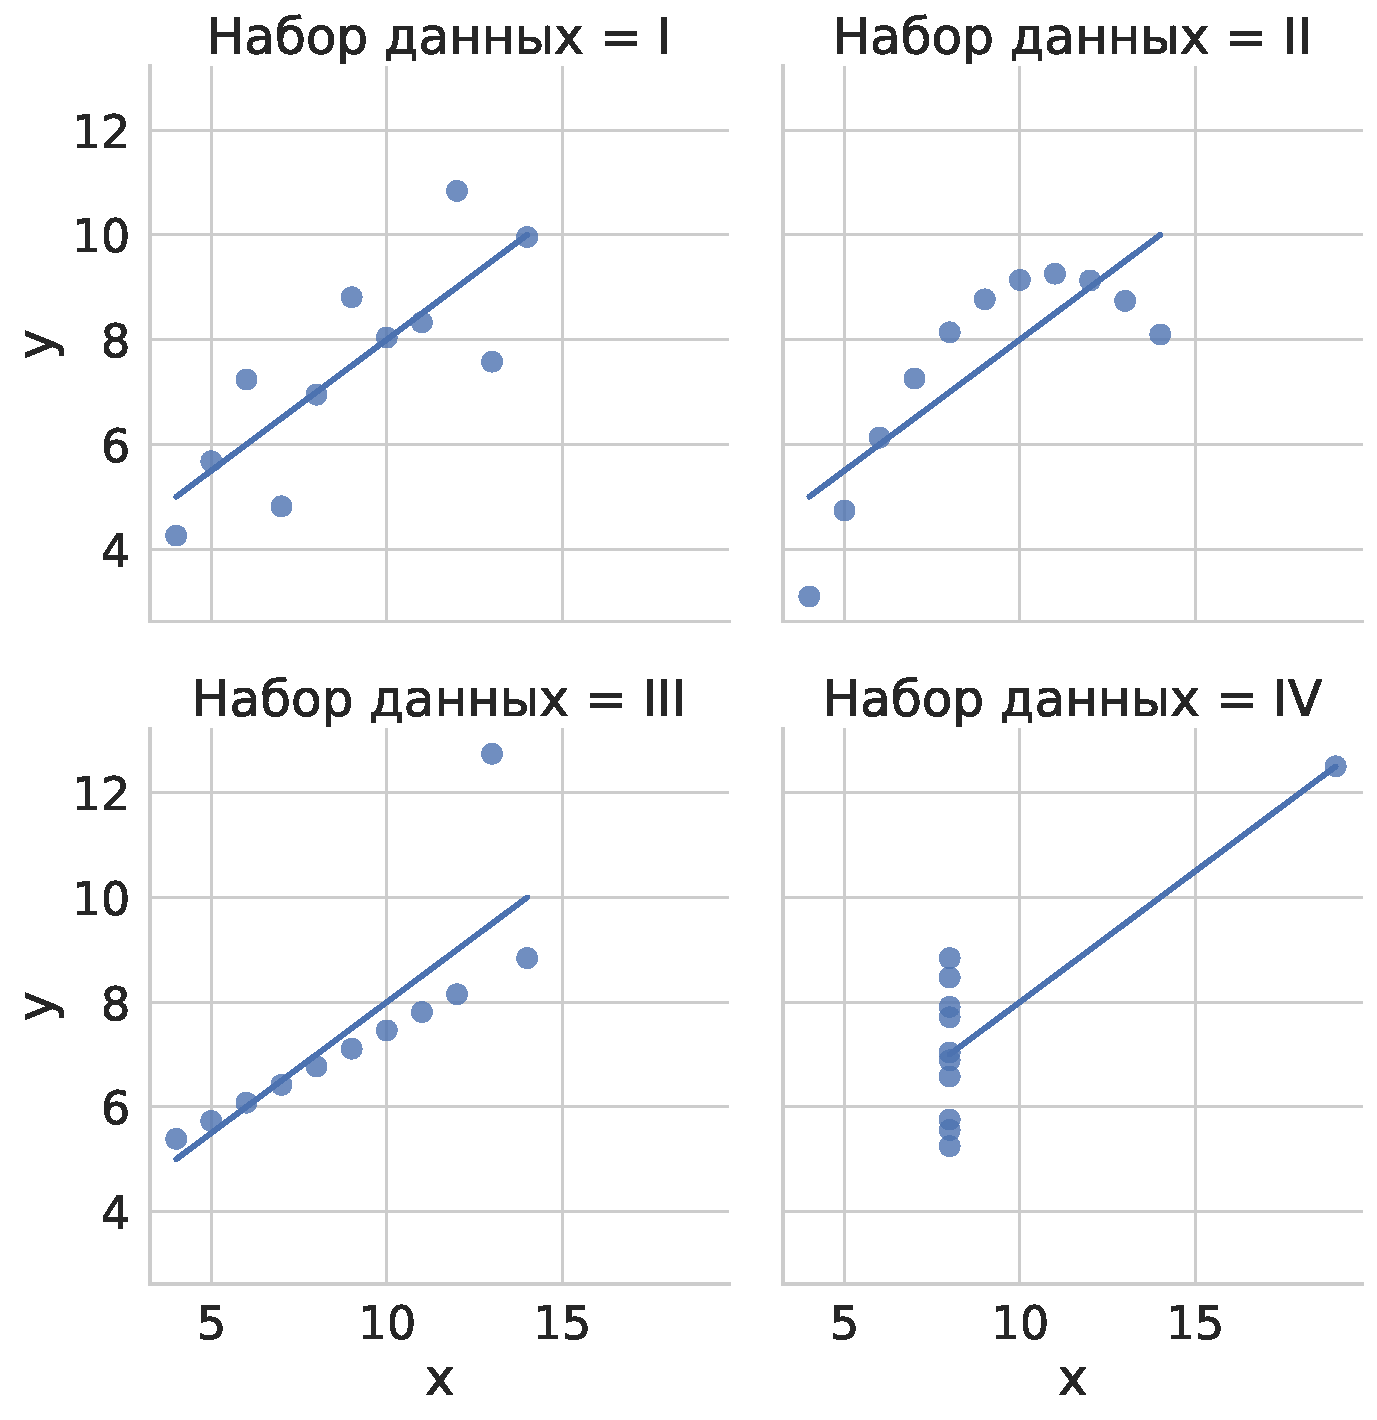
\includegraphics[width=0.7\textwidth]{anscombe_quartet}
        \caption{Квартет Энскомба.}
        \label{pic:anscombe_quartet}
    \end{figure}

    \begin{table}[!htp]
    	\centering
    	\caption{Статистические свойства наборов данных в Квартете Энскомба}
		\begin{tabular}{|l|l|}
			\hline
			Характеристика                         & Значение   \\ \hline
			Среднее значение переменной $x$        & 9.0        \\ \hline
			Дисперсия переменной $x$               & 10.0       \\ \hline
			Среднее значение переменной $y$        & 7.5        \\ \hline
			Дисперсия переменной $y$               & 3.75       \\ \hline
			Корреляция между переменными $x$ и $y$ & 0.816      \\ \hline
			Уравнение линейной регрессии           & $y=3+0.5x$ \\ \hline
			Коэффициент детерминации               & 0.67       \\
			линейной регрессии ($R^2$)             &            \\ \hline
		\end{tabular}
		\label{table:anscombe_quartet_statistics}
	\end{table}

	Что примечательно, все 4 подгруппы данных имеют одно и то же урванение 
	линейной регрессии (см. таблицу \ref{table:anscombe_quartet_statistics}) и, 
	как показано в таблице \ref{table:anscombe_quartet_rmse}, очень близкие 
	занчения корня из среднеквадратической ошибки.

	\begin{table}[!htp]
    	\centering
    	\caption{Значения корней из среднеквадратической ошибки}
		\begin{tabular}{|l|c|c|c|c|}
			\hline
			Набор данных                        & I     & II    & III   & IV    \\ \hline
			Значение корня среднеквадратической & 1.119 & 1.119 & 1.118 & 1.118 \\ 
			ошибки (RMSE)                       &       &       &       &       \\ \hline
		\end{tabular}
		\label{table:anscombe_quartet_rmse}
	\end{table}

	В таблице \ref{table:anscombe_quartet} для справки приведены данные из 
	<<Квартета Энскомба>>.

    \begin{table}[!htp]
    	\centering
    	\caption{Квартет Энскомба}
		\begin{tabular}{|ll|ll|ll|ll|}
			\hline
			\multicolumn{2}{|c|}{I}                             & \multicolumn{2}{c|}{II}                            & \multicolumn{2}{c|}{III}                           & \multicolumn{2}{c|}{IV}                            \\ \hline
			\multicolumn{1}{|c|}{x}    & \multicolumn{1}{c|}{y} & \multicolumn{1}{c|}{x}    & \multicolumn{1}{c|}{y} & \multicolumn{1}{c|}{x}    & \multicolumn{1}{c|}{y} & \multicolumn{1}{c|}{x}    & \multicolumn{1}{c|}{y} \\ \hline
			\multicolumn{1}{|l|}{10,0} & 8,04                   & \multicolumn{1}{l|}{10,0} & 9,14                   & \multicolumn{1}{l|}{10,0} & 7,46                   & \multicolumn{1}{l|}{8,0}  & 6,58                   \\ \hline
			\multicolumn{1}{|l|}{8,0}  & 6,95                   & \multicolumn{1}{l|}{8,0}  & 8,14                   & \multicolumn{1}{l|}{8,0}  & 6,77                   & \multicolumn{1}{l|}{8,0}  & 5,76                   \\ \hline
			\multicolumn{1}{|l|}{13,0} & 7,58                   & \multicolumn{1}{l|}{13,0} & 8,74                   & \multicolumn{1}{l|}{13,0} & 12,74                  & \multicolumn{1}{l|}{8,0}  & 7,71                   \\ \hline
			\multicolumn{1}{|l|}{9,0}  & 8,81                   & \multicolumn{1}{l|}{9,0}  & 8,77                   & \multicolumn{1}{l|}{9,0}  & 7,11                   & \multicolumn{1}{l|}{8,0}  & 8,84                   \\ \hline
			\multicolumn{1}{|l|}{11,0} & 8,33                   & \multicolumn{1}{l|}{11,0} & 9,26                   & \multicolumn{1}{l|}{11,0} & 7,81                   & \multicolumn{1}{l|}{8,0}  & 8,47                   \\ \hline
			\multicolumn{1}{|l|}{14,0} & 9,96                   & \multicolumn{1}{l|}{14,0} & 8,10                   & \multicolumn{1}{l|}{14,0} & 8,84                   & \multicolumn{1}{l|}{8,0}  & 7,04                   \\ \hline
			\multicolumn{1}{|l|}{6,0}  & 7,24                   & \multicolumn{1}{l|}{6,0}  & 6,13                   & \multicolumn{1}{l|}{6,0}  & 6,08                   & \multicolumn{1}{l|}{8,0}  & 5,25                   \\ \hline
			\multicolumn{1}{|l|}{4,0}  & 4,26                   & \multicolumn{1}{l|}{4,0}  & 3,10                   & \multicolumn{1}{l|}{4,0}  & 5,39                   & \multicolumn{1}{l|}{19,0} & 12,50                  \\ \hline
			\multicolumn{1}{|l|}{12,0} & 10,84                  & \multicolumn{1}{l|}{12,0} & 9,13                   & \multicolumn{1}{l|}{12,0} & 8,15                   & \multicolumn{1}{l|}{8,0}  & 5,56                   \\ \hline
			\multicolumn{1}{|l|}{7,0}  & 4,82                   & \multicolumn{1}{l|}{7,0}  & 7,26                   & \multicolumn{1}{l|}{7,0}  & 6,42                   & \multicolumn{1}{l|}{8,0}  & 7,91                   \\ \hline
			\multicolumn{1}{|l|}{5,0}  & 5,68                   & \multicolumn{1}{l|}{5,0}  & 4,74                   & \multicolumn{1}{l|}{5,0}  & 5,73                   & \multicolumn{1}{l|}{8,0}  & 6,89                   \\ \hline
		\end{tabular}
		\label{table:anscombe_quartet}
	\end{table}

	Квартет Энскомба -- не единственный набор данных, имеющий такие свойства, 
	но, пожалуй, самый известный \cite{anscombe_quartet_wikipedia}. 

	Конечно, достаточно просто построить график и попробовать идентифицировать
	разные виды моделей на одном и том же наборе данных, чтобы исключить такую
	ошибку и выбрать наиболее подходящие модели.

	
	Далее, обратимся к проблеме, называемой <<оверфитинг>>. Как уже было 
	сказано, оценка RMSE только на тренировочных данных -- методическая ошибка. 
	Если исследователь на этапе выбора модели (например, выбора между линейной
	и полиномиальной регрессией) или на этапе выбора параметров модели 
	(параметров, не зависящих от данных, например степени полинома) выполняет
	оценку данной метрики на том же наборе, на котором выполняет идентификацию 
	параметров модели, появляется риск настроить модель таким образом, что она 
	будет демонстрировать превосходные результаты на тренировочных данных 
	(показатель RMSE может буквально равняться нулю), но будет абсолютно 
	бесполезна на новых не входивших в тренировочный набор. Проще говоря, 
	появляется высокий риск выбрать слишком сложную модель, которая примет 
	случайные отклонения в тренировочных данных за закономеронсть, либо же 
	излишне адаптировать модель под тренировочный набор	\cite{hands_on_ml}, 
	\cite{nikolenko_deep_learning}.

	Для того чтобы проиллюстрировать эту проблему, подготовим небольшой набор
	данных, имитирующий результаты измерения величин $x$ и $y(x)$, связанных 
	выражением \ref{eq:fake_results}.
	\begin{equation}
		\label{eq:fake_results}
		y(x) = 1 + 0.5x + \epsilon,
	\end{equation}
	где $\epsilon$ -- нормально распределённая случайная величниа со средним,
	значением равным 0, и среднеквадратическим отклонением равным 0.4.
	В данном случае, зависимость $y(x)$ <<фундаментально>> линейна. Расчитаем
	для данной зависмости 10 точек в диапазоне от $x=0.5$ до $x=3.5$, затем, 
	выполним регрессию полученного набора данных линейной функцией и 
	алгебраическим полиномом десятой степени, в конце, оценим корень из
	среднеквадратической ошибки для обеих моделей. Рисунок 
	\ref{pic:overfitting_polynomial} демонстрирует результаты регрессий.

    \begin{figure}[!htp]
        \centering
        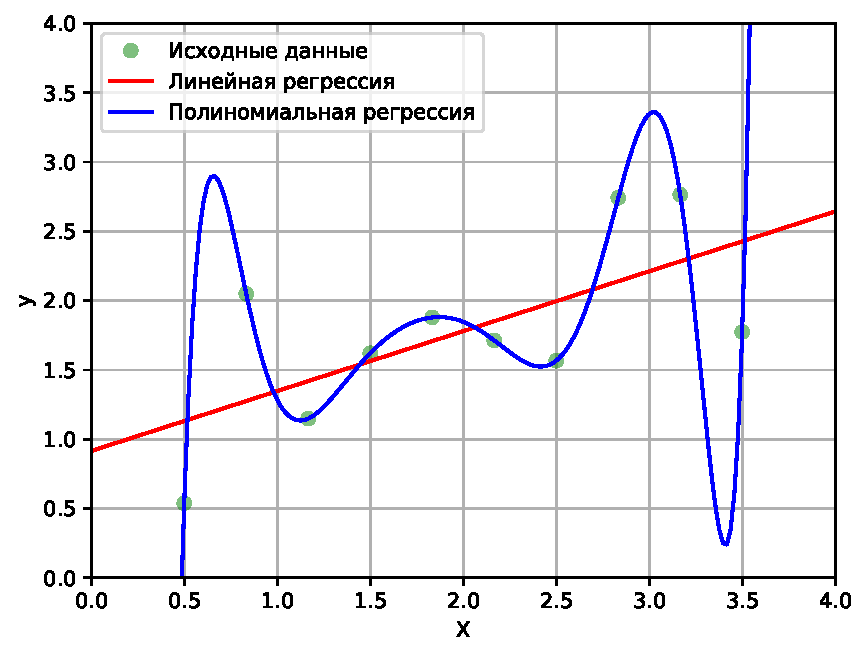
\includegraphics[width=0.5\textwidth]{overfitting_polynomial}
        \caption{Иллюстрация оверфитинга в случае полиномиальной модели.
                 Использовался полином десятой степени.}
        \label{pic:overfitting_polynomial}
    \end{figure}

    После идентификации для модели линейной регрессии получились следующие 
    параметры:
    \begin{description}
    	\item[a] -- коэффициент, характеризующий наклон, равен приблизительно 0.43;
    	\item[b] -- коэффициент, характеризующий смещение, равен приблизительно 0.92;
    	\item[RMSE] -- корень из среднеквадратической ошибки, равный приблизительно 0.48.
    \end{description}
    Как и ожидалось, полученные значения очень близки к параметрам выражения 
    \ref{eq:fake_results}.

    Не будем приводить все коэффициенты полиномиальной регрессии, корень из
    среднеквадратической ошибки для данной модели получился равным 
    $4.24 \cdot 10^{-11}$, на рисунке \ref{pic:overfitting_polynomial} видно, что
    график полиномиальной регрессии проходит через все точки исходных данных,
    при этом крайне маловероятно, что данная модель будет адекватно предсказывать
    значения $y(x)$, на значениях $x$, которых не было в тренировочном наборе.

    Для сравнения попробуем идентифицировать многоэкспоненциальную модель на 
    том же наборе данных, примем параметр n\_exps равным 10. Результаты 
    идентификации такой модели представлены на рисунке 
    \ref{pic:overfitting_multiexp}.

    \begin{figure}[!htp]
        \centering
        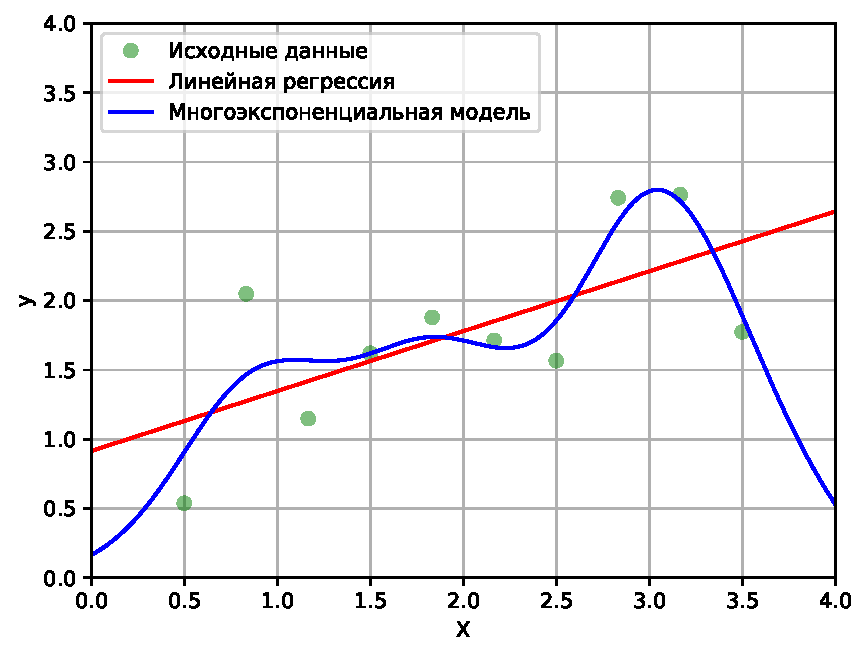
\includegraphics[width=0.5\textwidth]{overfitting_multiexp}
        \caption{Иллюстрация оверфитинга в случае многоэкспоненциальной модели.
                 Использовалась модель с параметром n\_exps = 10.}
        \label{pic:overfitting_multiexp}
    \end{figure}

    Для полученной многоэкспоненциальной модели с параметром n\_exps, равным 10
    корень из среднеквадратической ошибки получается приблизительно равным 0.28,
    что значительно больше, чем в случае полиномиальной регрессии, и всё еще 
    меньше, чем в случае линейной регрессии. При этом, хочется подчеркнуть, что
    данный набор точек является линейной функцией с добавлением нормально
    распределённой случайной составляющей (выражение \ref{eq:fake_results}).

    Существует несколько способов борьбы с оверфитингом, ниже приведены некоторые
    из них:
    \begin{itemize}
    	\item собрать больше данных (для того чтобы предыдущие примеры были 
    	показательны был намеренно сделан набор из 10 точек, получить аналогичный
    	эффект на наборе из 1000 точек сложнее);
    	\item использовать модель попроще;
    	\item использовать регуляризацию;
    	\item оценивать качество модели не на тренировочном наборе, а на отдельном
    	валидационном наборе (англ. validation set), случайно отобранной 
    	контрольной группе;
    	\item использовать приём, называемый кросвалидацией (англ. 
    	cross-validation) \cite{hands_on_ml}, \cite{sklearn_cross_validation}.
    \end{itemize}

    В задачах машинного обучения для того, чтобы оценить как точно модель 
    будет предсказывать целевые значения на новых данных, исходный набор 
    разделяют на две группы: тренировочную и тестовою. На тренировачном наборе
    данных проводится идентификация модели, а на тестовом только оценивают 
    качество самой финальной модели. Таким образом, применительно к задаче 
    регрессии, ожидается, что на новых, невходивших в тренировочный набор данных
    модель будет демонстрировать среднеквадратическую ошибку, близкую к 
    полученной на тестовом наборе.

    Если у модели есть параметр, не зависящий от данных, например, степень
    алгебраического полинома или количество экспоненциальных составляющих 
    многоэкспоненциальной модели (параметр n\_exps), и необходимо найти 
    оптимальное значение данного параметра, то из тренировочного набора выделяют
    еще один набор данных -- валидационный набор, на котором оценивают
    оценивают модель при каждом значении подстраемового параметра, в итоге
    выбор останавливают на параметре с которым модель показала лучший результат
    (наименьшее значение среднеквадратической ошибки). При этом модель не 
    тренируют на валидационном наборе, то есть тренировочный набор уменьшается.

    Подход с применением валидационного набора позволяет исключить оверфитинг 
    и прогнозировать эффективность модели. Однако, данный приём приводит к 
    сокращению тренировочных данных, что может вызывать проблемы в случаях 
    работы с наборами данных, содержащими небольшое количество наблюдений. В 
    таких случаях прибегают к технике, называемой кросвалидацией \cite{hands_on_ml}, 
    \cite{sklearn_cross_validation}.

    При использовании кросвалидации тестовый набор всё также применяется только
    для прогнозирования точности будующих предсказаний модели, на нем никогда 
    не производится обучение модели, и не производится оценка модели во время
    настройки её параметров. Тестовый набор же разбивается на $k$ подгрупп
    (в случае использования алгоритма k-fold cross-validation), затем модель
    в цикле из $k$ шагов обучают на $k-1$ подгруппах, а на оставшейся оценивают 
    модель (в случае регрессии считают среднеквадратическую ошибку), при этом 
    на каждом шаге цикла для оценки модели берут новую подгруппу. В конце 
    считают среднее значение метрики качества модели, полученной на каждом шаге
    цикла, это и будет результат кросвалидации. Таким образом, модель каждый 
    раз оценивается на данных, которые она <<не видела>> во время обучения, за
    счёт этого получается исключить использование валидационного набора, однако
    приходится тренировать модель k-раз \cite{sklearn_cross_validation}. 

    Рисунок \ref{pic:cross_val} демонстрирует схему работы с данных, при 
    применении кросвалидации. Зелёным отмечены наборы данных, на которых 
    проводится обучение модели, синим -- наборы, на которых выполняется оценка
    среднеквадратической ошибки \cite{sklearn_cross_validation}.

    \begin{figure}[!htp]
        \centering
        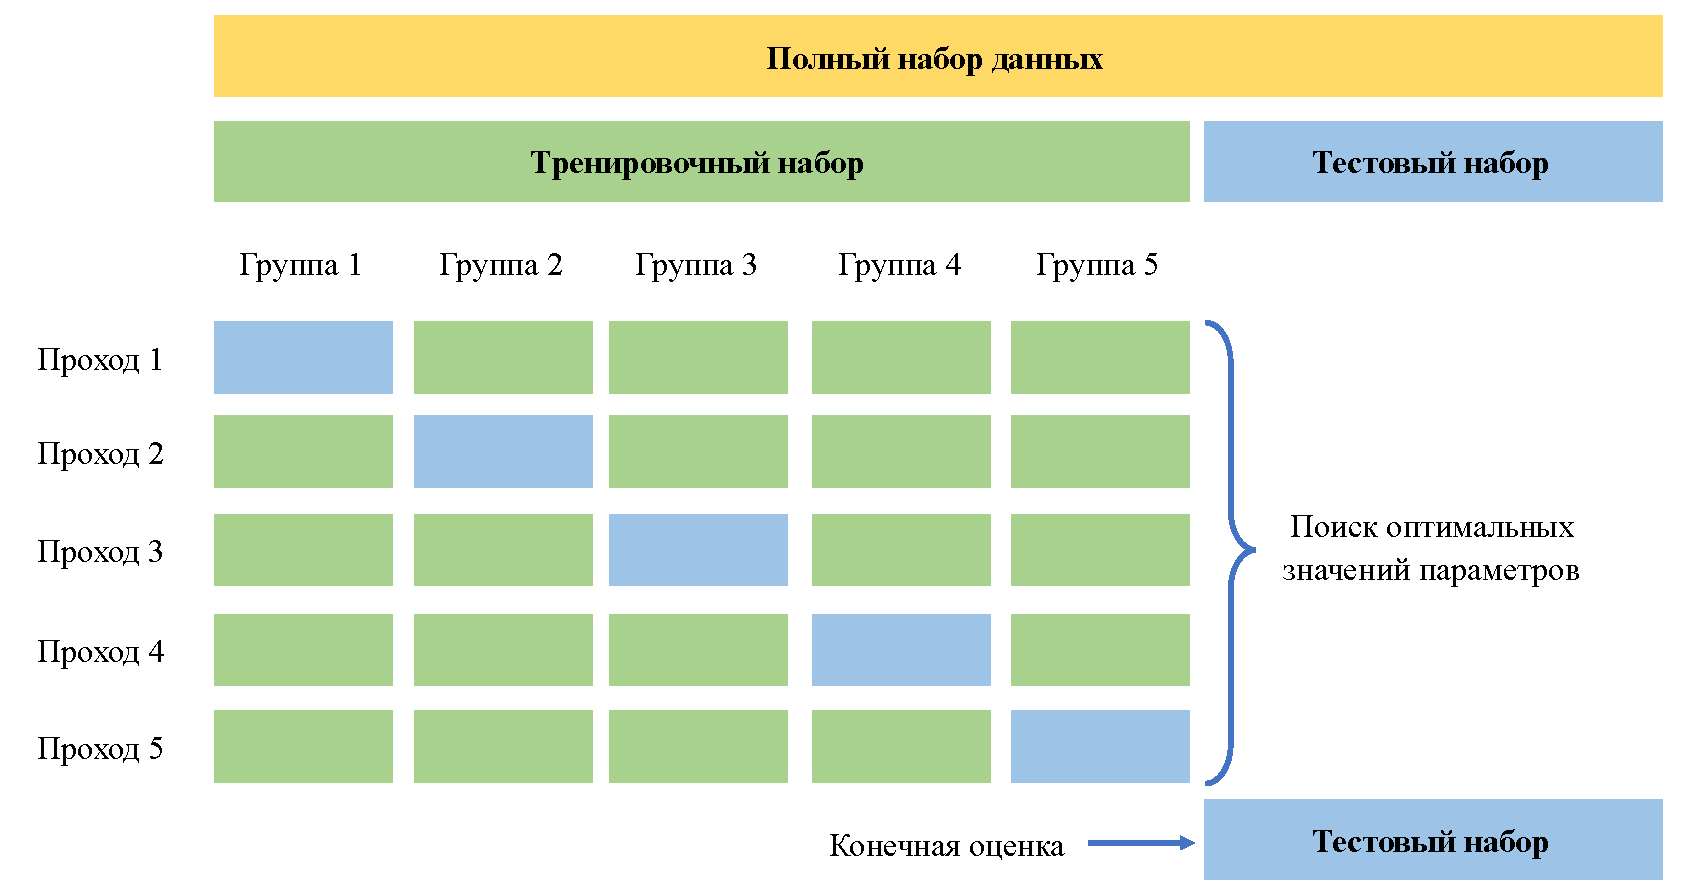
\includegraphics[width=0.75\textwidth]{cross_val}
        \caption{Иллюстрация кросвалидации.}
        \label{pic:cross_val}
    \end{figure}

    При оптимизации патаметров модели, не зависящих от данных, по сути, 
    параметров алгоритма идентификации, например количество экспоненциальных 
    составляющих многоэксопоненциальной модели, кросвалидацию выполняют для 
    каждого комплекта значений параметров и выбирают комплект, с которым 
    модель показала лучший результат (такая техника оптимизации в англоязычной 
    литературе называется <<grid search>>, то есть поиск по сетке). В конце,
    модель с победившим набором параметров еще раз идентифицируют на полном
    тренировочном наборе данных, после этого, если разработка модели закончена
    можно выполнить оценку на тестовом наборе \cite{sklearn_cross_validation}.

    Таким образом, при оценке модели не стоит ограничиваться только расчётом
    среднеквадратической ошибки, целесообразно строить графики, применять 
    дополнительные приёмы и метрики, которые на самом деле не ограничиваются
    названными в данном разделе. 

    В следующем разделе мы апробуем разработанные модели на экспериментальных 
    данных и сравним результаты для разных моделей.